\documentclass[10pt,a4paper]{article}
\usepackage[margin=30mm]{geometry}
\usepackage{amsmath,fancyvrb,float,hyperref,structmech}
\usepackage{mathpazo}
\title{structmech\\\large{}A TikZ command set for structural mechanics drawings}
\author{Theodore Chang\footnote{E-mail: \href{tlcfem@gmail.com}{tlcfem@gmail.com}}\\[2mm]\normalsize{}University of Canterbury, Christchurch, NZ}
\date{\normalsize{}v1.0 released on \today}
\newcommand*{\Highlight}[1]{\colorbox{cyan}{\color{red}\texttt{#1}}}
\begin{document}
\maketitle
\section{Introduction}
When I was preparing lecture notes on structural mechanics related topics, it took me a lot of time to draw simple beam systems and distributions of internal forces, such as shear force diagram (SFD) and bending moment diagram (BMD), using basic TikZ. I thus tried to write some generalised commands that can draw key elements with simple syntax. That's how this package is created. This package is under GPL v3 license and/or later version. Please feel free to redistribute, expand or rewrite the functionality.
\section{Options}
To load the package, please use the following command in the preamble.
\begin{Verbatim}[frame=single,label=Syntax]
\usepackage[key=val]{structmech}
\end{Verbatim}
Some options are available for controlling the parameters used during plotting, they are:
\begin{enumerate}
\item \Highlight{fill} defines the default fill patch colour, any predefined colour value is acceptable.
\item \Highlight{line} defines the default line colour, any predefined colour value is acceptable.
\item \Highlight{node} defines the nodal force/displacement colour, any predefined colour value is acceptable.
\item \Highlight{axis} defines the axial force/displacement colour, any predefined colour value is acceptable.
\item \Highlight{rotation} defines the rotation force/displacement colour, any predefined colour value is acceptable.
\item \Highlight{convention} defines the sign convention, value \Highlight{convention=sign} draws all quantities along the positive direction and indicates the negative quantities with minus sign $-$, value \Highlight{convention=direction} labels all numbers as positive values but draws the negative quantities along the negative direction.
\item \Highlight{showvalue} defines whether to show the values when plotting the diagrams of the internal forces, possible values are \Highlight{showvalue=on} and \Highlight{showvalue=off}.
\item \Highlight{absvalue} defines whether to show the absolute values when plotting the diagrams of the internal forces, possible values are \Highlight{absvalue=on} and \Highlight{absvalue=off}.
\item \Highlight{opacity} defines the fill patch opacity, default value is $0.4$.
\item \Highlight{linewidth} defines the line width, default value is $0.4$ millimetre.
\end{enumerate}
These options can be changed in the document via the following command.
\begin{Verbatim}[frame=single,label=Syntax]
\setstructmech{key=val}
\end{Verbatim}
Here are some examples that use the basic force command to show how the user can control the property of the diagram elements. Other options can be changed in a similar fashion.
\begin{Verbatim}[frame=single,label=Example]
\setstructmech{axis=red}
\BasicForce{0,0}{3,0}{}
\setstructmech{axis=blue,rotation=green}
\BasicForce{4,0}{7,0}{}
\setstructmech{axis=black}
\BasicForce{8,0}{11,0}{}
\end{Verbatim}
\begin{figure}[H]
\centering
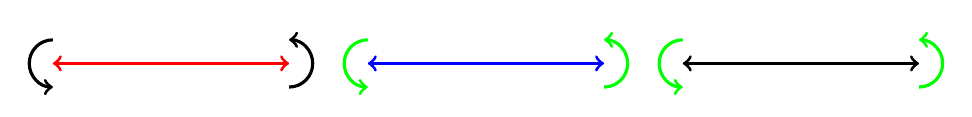
\begin{tikzpicture}
\setstructmech{axis=red}
\BasicForce{0,0}{3,0}{}
\setstructmech{axis=blue,rotation=green}
\BasicForce{4,0}{7,0}{}
\setstructmech{axis=black}
\BasicForce{8,0}{11,0}{}
\end{tikzpicture}
\end{figure}
\section{Nodal Forces/Displacements}
\begin{Verbatim}[frame=single,label=Syntax]
\NodalForce[1]{2}[3][4][5]{6}[7]
\end{Verbatim}
\begin{itemize}
\item[][1] --- optional, colour of arrows, any existing colour value is acceptable, default value is the colour defined by the \Highlight{node} option.
\item[]\{2\} --- node coordinate pair, accepts two coordinates of the target node in the form of \Highlight{$x,y$}.
\item[][3] --- optional, label for local horizontal force/displacement, if not assigned or left blank, only the arrow (without label) will be drew, assign \Highlight{N} for drawing nothing along horizontal direction.
\item[][4] --- optional, label for local vertical force/displacement, if not assigned or left blank, only the arrow (without label) will be drew, assign \Highlight{N} for drawing nothing along horizontal direction.
\item[][5] --- optional, label for local rotational force/displacement, if not assigned or left blank, only the arrow (without label) will be drew, assign \Highlight{N} for drawing nothing along horizontal direction.
\item[]\{6\} --- optional, rotation, default value is \Highlight{$0$}.
\item[][7] --- optional, scale, default value is \Highlight{$1$}.
\end{itemize}
\begin{Verbatim}[frame=single,label=Example]
\NodalForce{0,0}
\NodalForce[red]{2,0}
\NodalForce[blue]{4,0}[][][]
\setstructmech{node=green}
\NodalForce{6,0}[N]
\NodalForce{8,0}[][N]
\NodalForce{10,0}[][][N]
\NodalForce{12,0}[N][]
\setstructmech{node=orange}
\setstructmech{convention=direction}
\NodalForce{0,-3}[-V_1][-V_2][-V_3]
\setstructmech{convention=sign}
\NodalForce{2.5,-3}[-V_1][-V_2][-V_3]
\NodalForce{4.5,-3}[V_1][V_2][V_3]{60}
\NodalForce{7,-3}{150}[1.3]
\NodalForce{9,-3}[N][V_2]{90}[1.6]
\NodalForce[cyan]{12.5,-4}[V_1][V_2][V_3]{-60}[2]
\end{Verbatim}
\begin{figure}[H]
\centering
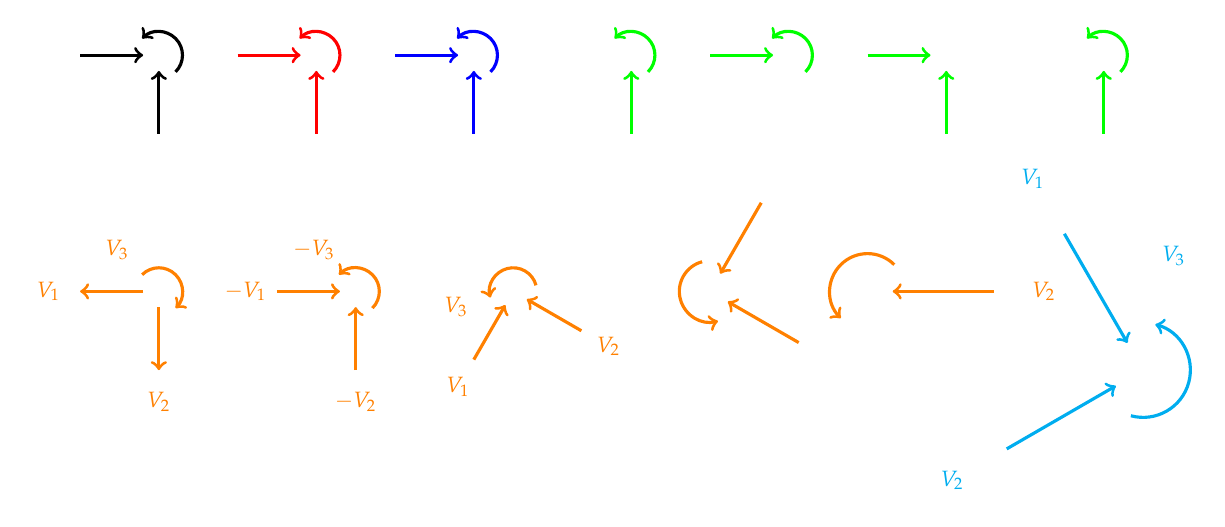
\begin{tikzpicture}
\NodalForce{0,0}
\NodalForce[red]{2,0}
\NodalForce[blue]{4,0}[][][]
\setstructmech{node=green}
\NodalForce{6,0}[N]
\NodalForce{8,0}[][N]
\NodalForce{10,0}[][][N]
\NodalForce{12,0}[N][]
\setstructmech{node=orange}
\setstructmech{convention=direction}
\NodalForce{0,-3}[-V_1][-V_2][-V_3]
\setstructmech{convention=sign}
\NodalForce{2.5,-3}[-V_1][-V_2][-V_3]
\NodalForce{4.5,-3}[V_1][V_2][V_3]{60}
\NodalForce{7,-3}{150}[1.3]
\NodalForce{9,-3}[N][V_2]{90}[1.6]
\NodalForce[cyan]{12.5,-4}[V_1][V_2][V_3]{-60}[2]
\end{tikzpicture}
\end{figure}
\section{Member Forces/Displacements}
\begin{Verbatim}[frame=single,label=Syntax]
\BasicForce[1]{2}{3}{4}{5}[6][7][8]
\end{Verbatim}
\begin{enumerate}
\item[][1] --- optional, the number of forces to draw, \Highlight{1} for axial force only, \Highlight{2L} for lower end bending moment only, \Highlight{2H} for high end bending moment only, \Highlight{2} for both two end moments, \Highlight{3} for all three force components, default value is \Highlight{3}.
\item[]\{2\} --- the coordinates of the lower end in the form of \Highlight{$x,y$}.
\item[]\{3\} --- the coordinates of the high end in the form of \Highlight{$x,y$}.
\item[]\{4\} --- label for the member, leave blank if not required.
\item[]\{5\} --- optional, further adjustment of the member label, parameters used for TikZ positioning are acceptable, such as \Highlight{right=2mm} or \Highlight{anchor=north}, the default value is \Highlight{above=2mm}, leave blank if not required.
\item[][6] --- label for the first force drew, available for all four values for the first parameter \Highlight{\#1}, leave blank if not required.
\item[][7] --- label for the second force drew, available for \Highlight{\#1=2}, leave blank if not required.
\item[][8] --- label for the third force drew, available for \Highlight{\#1=3}, leave blank if not required.
\end{enumerate}
The colours of three components can be configured using global options. Here are a few examples, please find out the order and the difference in the following fourteen examples.
\begin{Verbatim}[frame=single,label=Example]
\BasicForce{0,0}{3,0}{}
\BasicForce[1]{5,0}{8,0}{a}[U_1]
\BasicForce[1]{0,2}{3,2}{}
\BasicForce[2]{5,2}{8,2}{a}[U_1][U_2]
\setstructmech{axis=red,rotation=green}
\BasicForce[2]{0,4}{3,4}{}
\BasicForce[2L]{5,4}{8,4}{a}[U_1]
\BasicForce[3]{0,6}{3,6}{}
\BasicForce[2H]{5,6}{8,6}{a}[U_1]
\BasicForce[2L]{0,8}{3,8}{}
\BasicForce{5,8}{8,8}{a}[U_1][U_2][U_3]
\BasicForce[2H]{0,10}{3,10}{}
\BasicForce{5,10}{8,10}{a}{above left=2mm and 6mm}[U_1][U_2][U_3]
\setstructmech{convention=direction}
\BasicForce[3]{0,12}{3,12}{a}[-U_1][-U_2][-U_3]
\BasicForce[3]{5,12}{8,12}{a}[U_1][U_2][-U_3]
\end{Verbatim}
\begin{figure}[H]
\centering
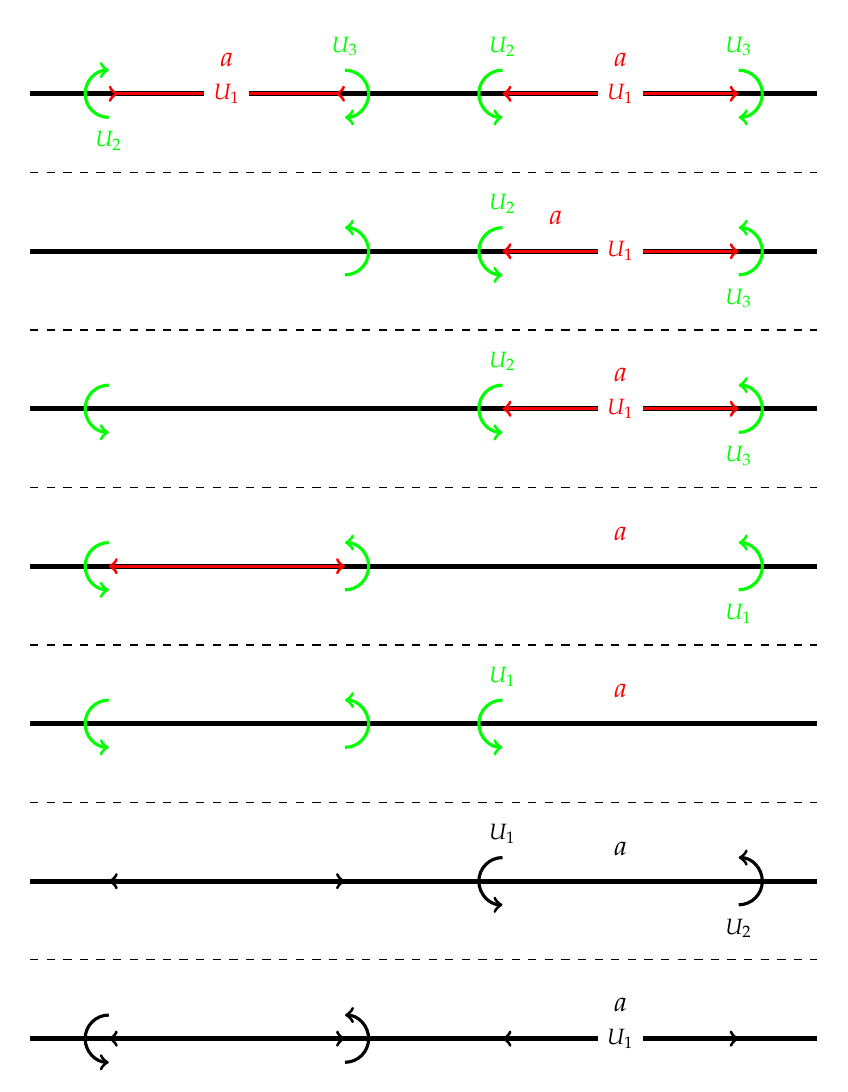
\begin{tikzpicture}
\draw[dashed](-1,1)--(9,1)(-1,3)--(9,3)(-1,5)--(9,5)(-1,7)--(9,7)(-1,9)--(9,9)(-1,11)--(9,11);
\draw[line width=.6mm](-1,0)--(9,0)(-1,2)--(9,2)(-1,4)--(9,4)(-1,6)--(9,6)(-1,8)--(9,8)(-1,10)--(9,10)(-1,12)--(9,12);
\BasicForce{0,0}{3,0}{}
\BasicForce[1]{5,0}{8,0}{a}[U_1]
\BasicForce[1]{0,2}{3,2}{}
\BasicForce[2]{5,2}{8,2}{a}[U_1][U_2]
\setstructmech{axis=red,rotation=green}
\BasicForce[2]{0,4}{3,4}{}
\BasicForce[2L]{5,4}{8,4}{a}[U_1]
\BasicForce[3]{0,6}{3,6}{}
\BasicForce[2H]{5,6}{8,6}{a}[U_1]
\BasicForce[2L]{0,8}{3,8}{}
\BasicForce{5,8}{8,8}{a}[U_1][U_2][U_3]
\BasicForce[2H]{0,10}{3,10}{}
\BasicForce{5,10}{8,10}{a}{above left=2mm and 6mm}[U_1][U_2][U_3]
\setstructmech{convention=direction}
\BasicForce[3]{0,12}{3,12}{a}[-U_1][-U_2][-U_3]
\BasicForce[3]{5,12}{8,12}{a}[U_1][U_2][-U_3]
\end{tikzpicture}
\end{figure}
\section{Uniformly Distributed Load}
\begin{Verbatim}[frame=single,label=Syntax]
\UDL[1]{2}{3}[4]{5}
\end{Verbatim}
\begin{enumerate}
\item[][1] --- optional, flip the side, assign value \Highlight{F} if the default behaviour is not the one you want.
\item[]\{2\} --- the coordinates of the lower end node in form of \Highlight{$x,y$}.
\item[]\{3\} --- the coordinates of the higher end node in form of \Highlight{$x,y$}.
\item[][4] --- optional, label.
\item[]\{5\} --- optional, scale, default value is \Highlight{$1$}.
\end{enumerate}
\begin{Verbatim}[frame=single,label=Example]
\UDL{-4,0}{-1,4}[10]
\UDL{-2,0}{1,4}[-10]
\setstructmech{fill=red,convention=direction}
\UDL{0,0}{3,4}[-10]
\setstructmech{fill=red,convention=sign}
\UDL[F]{1,0}{4,4}
\UDL{6,0}{9,4}{2}
\end{Verbatim}
\begin{figure}[H]
\centering
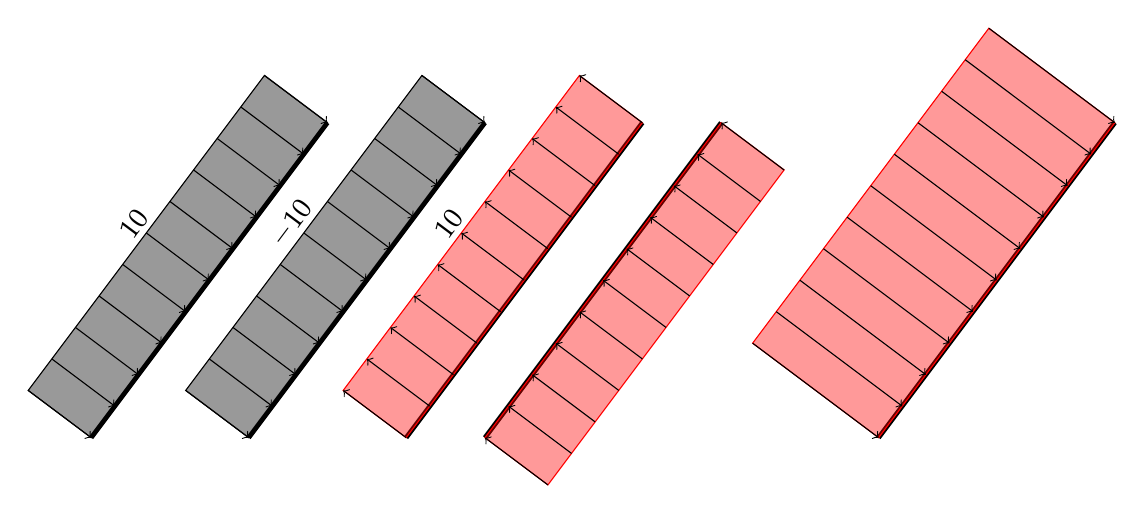
\begin{tikzpicture}
\draw[line width=.6mm](-4,0)--++(3,4)(-2,0)--++(3,4)(0,0)--++(3,4)(1,0)--++(3,4)(6,0)--++(3,4);
\UDL{-4,0}{-1,4}[10]
\UDL{-2,0}{1,4}[-10]
\setstructmech{fill=red,convention=direction}
\UDL{0,0}{3,4}[-10]
\setstructmech{fill=red,convention=sign}
\UDL[F]{1,0}{4,4}
\UDL{6,0}{9,4}{2}
\end{tikzpicture}
\end{figure}
\section{Supports}
\subsection{Hinge/Fixed/Roller/Slider Support}
\begin{Verbatim}[frame=single,label=Syntax]
\HingeSupport[1]{2}{3}
\FixedSupport[1]{2}{3}
\RollerSupport[1]{2}{3}
\SliderSupport[1]{2}{3}
\end{Verbatim}
\begin{enumerate}
\item[][1] --- optional, rotation, default value is \Highlight{$0$}.
\item[]\{2\} --- node coordinates in form of \Highlight{$x,y$}.
\item[]\{3\} --- optional, scale, default value is \Highlight{$1$}.
\end{enumerate}
\begin{Verbatim}[frame=single,label=Example]
\HingeSupport{0,0}
\HingeSupport[75]{2,0}{1.5}
\HingeSupport[150]{2,2}{2}
\HingeSupport[225]{0,2}{2.5}
\FixedSupport{4,0}
\FixedSupport[75]{6,0}{1.5}
\FixedSupport[150]{6,2}{2}
\FixedSupport[225]{4,2}{2.5}
\setstructmech{linewidth=.2mm,line=red}
\RollerSupport{6,-5}
\RollerSupport[75]{8,-5}{1.5}
\RollerSupport[150]{8,-3}{2}
\RollerSupport[225]{6,-3}{2.5}
\SliderSupport{0,-5}
\SliderSupport[75]{2,-5}{1.5}
\SliderSupport[150]{2,-3}{2}
\SliderSupport[225]{0,-3}{2.5}
\end{Verbatim}
\begin{figure}[H]
\centering
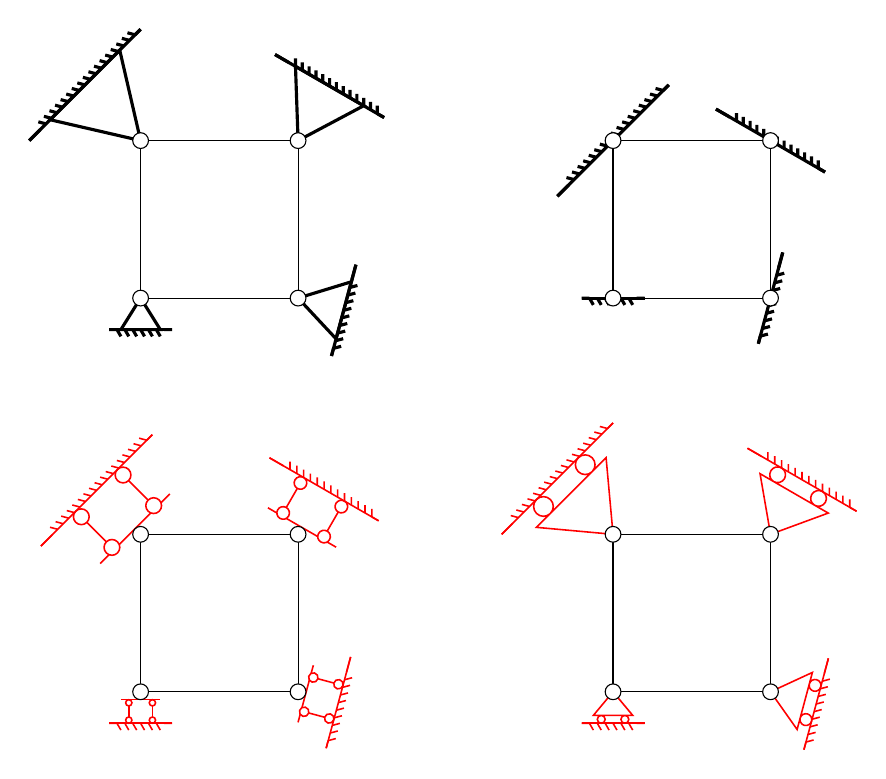
\begin{tikzpicture}
\HingeSupport{0,0}
\HingeSupport[75]{2,0}{1.5}
\HingeSupport[150]{2,2}{2}
\HingeSupport[225]{0,2}{2.5}
\draw
	(0,0)node[draw,fill=white,circle,inner sep=0,minimum size=2mm]{}--
	(2,0)node[draw,fill=white,circle,inner sep=0,minimum size=2mm]{}--
	(2,2)node[draw,fill=white,circle,inner sep=0,minimum size=2mm]{}--
	(0,2)node[draw,fill=white,circle,inner sep=0,minimum size=2mm]{}--cycle;
\FixedSupport{6,0}
\FixedSupport[75]{8,0}{1.5}
\FixedSupport[150]{8,2}{2}
\FixedSupport[225]{6,2}{2.5}
\setstructmech{linewidth=.2mm,line=red}
\draw
	(6,0)node[draw,fill=white,circle,inner sep=0,minimum size=2mm]{}--
	(8,0)node[draw,fill=white,circle,inner sep=0,minimum size=2mm]{}--
	(8,2)node[draw,fill=white,circle,inner sep=0,minimum size=2mm]{}--
	(6,2)node[draw,fill=white,circle,inner sep=0,minimum size=2mm]{}--cycle;
\RollerSupport{6,-5}
\RollerSupport[75]{8,-5}{1.5}
\RollerSupport[150]{8,-3}{2}
\RollerSupport[225]{6,-3}{2.5}
\draw
	(6,-5)node[draw,fill=white,circle,inner sep=0,minimum size=2mm]{}--
	(8,-5)node[draw,fill=white,circle,inner sep=0,minimum size=2mm]{}--
	(8,-3)node[draw,fill=white,circle,inner sep=0,minimum size=2mm]{}--
	(6,-3)node[draw,fill=white,circle,inner sep=0,minimum size=2mm]{}--cycle;
\SliderSupport{0,-5}
\SliderSupport[75]{2,-5}{1.5}
\SliderSupport[150]{2,-3}{2}
\setstructmech{linewidth=.2mm}
\SliderSupport[225]{0,-3}{2.5}
\draw
	(0,-5)node[draw,fill=white,circle,inner sep=0,minimum size=2mm]{}--
	(2,-5)node[draw,fill=white,circle,inner sep=0,minimum size=2mm]{}--
	(2,-3)node[draw,fill=white,circle,inner sep=0,minimum size=2mm]{}--
	(0,-3)node[draw,fill=white,circle,inner sep=0,minimum size=2mm]{}--cycle;
\end{tikzpicture}
\end{figure}
\subsection{Sleeve Support}
\begin{Verbatim}[frame=single,label=Syntax]
\SleeveSupport[1]{2}[3]{4}
\end{Verbatim}
\begin{enumerate}
\item[][1] --- optional, rotation.
\item[]\{2\} --- node coordinates in form of \Highlight{$x,y$}.
\item[][3] --- optional, gap width.
\item[]\{4\} --- optional, scale.
\end{enumerate}
\begin{Verbatim}[frame=single,label=Example]
\SleeveSupport{0,0}
\SleeveSupport[75]{2,0}{1.5}
\SleeveSupport[150]{2,2}{2}
\SleeveSupport[225]{0,2}[.12]{2.5}
\end{Verbatim}
\begin{figure}[H]
\centering
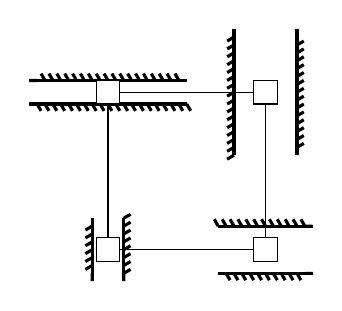
\begin{tikzpicture}
\SleeveSupport{0,0}
\SleeveSupport[90]{2,0}{1.5}
\SleeveSupport[180]{2,2}{2}
\SleeveSupport[270]{0,2}[.12]{2.5}
\draw
	(0,0)node[draw,fill=white,inner sep=0,minimum size=3mm]{}--
	(2,0)node[draw,fill=white,inner sep=0,minimum size=3mm]{}--
	(2,2)node[draw,fill=white,inner sep=0,minimum size=3mm]{}--
	(0,2)node[draw,fill=white,inner sep=0,minimum size=3mm]{}--cycle;
\end{tikzpicture}
\end{figure}
\subsection{Rigid Constraint}
\begin{Verbatim}[frame=single,label=Syntax]
\Rigid[1]{2}{3}
\end{Verbatim}
\begin{enumerate}
\item[][1] --- optional, rotation.
\item[]\{2\} --- node coordinates in form of \Highlight{$x,y$}.
\item[]\{3\} --- optional, scale.
\end{enumerate}
The colour is controlled by the \Highlight{fill} option instead of the \Highlight{line} option due to the fill patch is used in this command.
\begin{Verbatim}[frame=single,label=Example]
\Rigid{0,0}
\Rigid[-90]{2,0}{1.5}
\setstructmech{fill=yellow}
\Rigid[0]{2,2}{2}
\Rigid[90]{0,2}{2.5}
\end{Verbatim}
\begin{figure}[H]
\centering
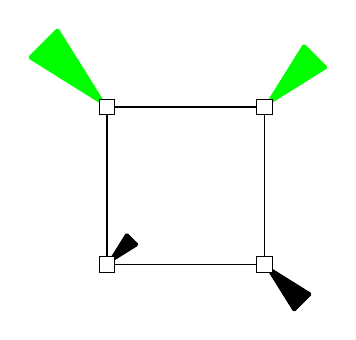
\begin{tikzpicture}
\Rigid{0,0}
\Rigid[-90]{2,0}{1.5}
\setstructmech{fill=green}
\Rigid[0]{2,2}{2}
\Rigid[90]{0,2}{2.5}
\draw
	(0,0)node[draw,fill=white,inner sep=0,minimum size=2mm]{}--
	(2,0)node[draw,fill=white,inner sep=0,minimum size=2mm]{}--
	(2,2)node[draw,fill=white,inner sep=0,minimum size=2mm]{}--
	(0,2)node[draw,fill=white,inner sep=0,minimum size=2mm]{}--cycle;
\end{tikzpicture}
\end{figure}
\section{Coordinate System Frame}
\begin{Verbatim}[frame=single,label=Syntax]
\CoorOrigin[1]{2}[3][4]{5}
\end{Verbatim}
\begin{enumerate}
\item[][1] --- optional, rotation, default value is \Highlight{$0$}.
\item[]\{2\} --- node coordinates in form of \Highlight{$x,y$}.
\item[][3] --- optional, label for $x$ axis, default value is \Highlight{$x$}.
\item[][4] --- optional, label for $y$ axis, default value is \Highlight{$y$}.
\item[]\{5\} --- optional, scale.
\end{enumerate}
\begin{Verbatim}[frame=single,label=Example]
\CoorOrigin{0,0}
\CoorOrigin[75]{4,0}[\xi][\eta]{1.5}
\CoorOrigin[150]{8,0}{2}
\CoorOrigin[225]{12,0}{2.5}
\end{Verbatim}
\begin{figure}[H]
\centering
\begin{tikzpicture}
\CoorOrigin{0,0}
\CoorOrigin[75]{4,0}[\xi][\eta]{1.5}
\CoorOrigin[150]{8,0}{2}
\CoorOrigin[225]{12,0}[x(\xi)][y(\eta)]{2.5}
\end{tikzpicture}
\end{figure}
\section{Internal Force Diagram}
\subsection{Linear Internal Force}
\begin{Verbatim}[frame=single,label=Syntax]
\IForceA[1]{2}{3}{4}{5}{6}
\end{Verbatim}
\begin{enumerate}
\item[][1] --- optional, fill colour.
\item[]\{2\} --- node coordinates of the lower end in form of \Highlight{$x,y$}.
\item[]\{3\} --- node coordinates of the higher end in form of \Highlight{$x,y$}.
\item[]\{4\} --- force value of the lower end, can be negative.
\item[]\{5\} --- force value of the higher end, can be negative.
\item[]\{6\} --- optional, scale.
\end{enumerate}
Caveat: it shall be noted that all internal forces follow the sign convention that is adopted in finite element method, instead of the one used in material mechanics. All quantities are defined in the local coordinate system.
\begin{Verbatim}[frame=single,label=Example]
\IForceA{0,0}{0,4}{1}{-2}
\setstructmech{absvalue=on}
\IForceA[blue]{0,4}{4,4}{2}{-0.5}{0.5}
\IForceA[cyan]{4,4}{4,0}{0.5}{2}
\setstructmech{showvalue=off,opacity=.8}
\IForceA[red]{4,0}{0,0}{-1}{-1}
\end{Verbatim}
\begin{figure}[H]
\centering
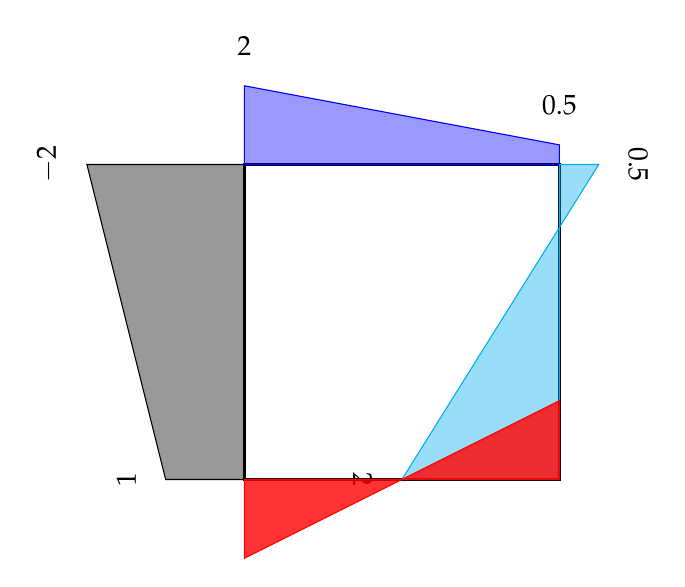
\begin{tikzpicture}
\draw[line width=.4mm](0,0)rectangle(4,4);
\IForceA{0,0}{0,4}{1}{-2}
\setstructmech{absvalue=on}
\IForceA[blue]{0,4}{4,4}{2}{-0.5}{0.5}
\IForceA[cyan]{4,4}{4,0}{0.5}{2}
\setstructmech{showvalue=off,opacity=.8}
\IForceA[red]{4,0}{0,0}{-1}{-1}
\end{tikzpicture}
\end{figure}
\subsection{Parabolic Internal Force}
\begin{Verbatim}[frame=single,label=Syntax]
\IForceB[1]{2}{3}{4}{5}{6}{7}
\end{Verbatim}
\begin{enumerate}
\item[][1] --- optional, fill colour.
\item[]\{2\} --- node coordinates of the lower end in form of \Highlight{$x,y$}.
\item[]\{3\} --- node coordinates of the higher end in form of \Highlight{$x,y$}.
\item[]\{4\} --- bending moment value of the lower end, can be negative.
\item[]\{5\} --- bending moment value of the higher end, can be negative.
\item[]\{6\} --- the increment of the moment value of the centre point.
\item[]\{7\} --- optional, scale.
\end{enumerate}
It should be noted that parameter \Highlight{\#6} defines the difference of the true moment value and the corresponding value of an assumed linear distribution. The positive value indicates that the parabola bends towards the local positive direction. Since this command draws a parabola, the load should be a uniformly distributed load. So this value \Highlight{\#6} is $\pm\dfrac{wl^2}{8}$, the sign depends on the direction of the UDL.
\begin{Verbatim}[frame=single,label=Example]
\draw[line width=.4mm](0,0)rectangle(4,4);
\IForceB{0,0}{0,4}{1}{-4}{1}{0.5}
\IForceB[red]{0,4}{4,4}{-2}{-1}{-2}{0.5}
\setstructmech{absvalue=on}
\IForceB[purple]{4,4}{4,0}{3}{-1}{2}{0.5}
\setstructmech{showvalue=off,opacity=.8}
\IForceB[cyan]{4,0}{0,0}{1.5}{0}{2}{0.5}
\end{Verbatim}
\begin{figure}[H]
\centering
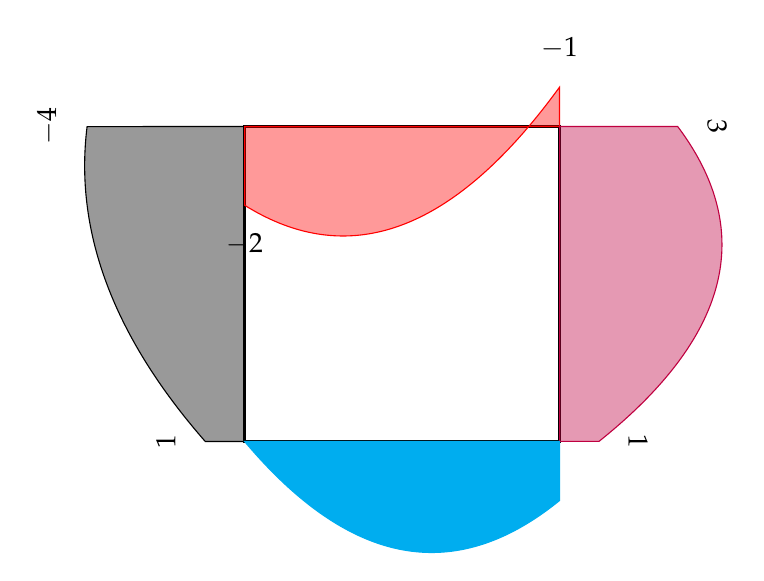
\begin{tikzpicture}
\draw[line width=.4mm](0,0)rectangle(4,4);
\IForceB{0,0}{0,4}{1}{-4}{1}{0.5}
\IForceB[red]{0,4}{4,4}{-2}{-1}{-2}{0.5}
\setstructmech{absvalue=on}
\IForceB[purple]{4,4}{4,0}{3}{-1}{2}{0.5}
\setstructmech{showvalue=off,opacity=1}
\IForceB[cyan]{4,0}{0,0}{1.5}{0}{2}{0.5}
\end{tikzpicture}
\end{figure}
\section{Beam Deformation (Perpendicular)}
\begin{Verbatim}[frame=single,label=Syntax]
\BeamDeformP[1]{2}{3}{4}[5]{6}[7]{8}
\end{Verbatim}
\begin{enumerate}
\item[][1] --- optional, line colour.
\item[]\{2\} --- node coordinates of the lower end in form of \Highlight{$x,y$}.
\item[]\{3\} --- node coordinates of the higher end in form of \Highlight{$x,y$}.
\item[]\{4\} --- perpendicular displacement of the lower end, can be negative, leave zero if not required.
\item[][5] --- optional, rotation value of the lower end, can be negative.
\item[]\{6\} --- perpendicular displacement of the high end, can be negative, leave zero if not required.
\item[][7] --- optional, rotation value of the high end, can be negative.
\item[]\{8\} --- optional, scale.
\end{enumerate}
Caveat: This command draws deformation based on local coordinate system. The translations are perpendicular to the member cord.
\begin{Verbatim}[frame=single,label=Example]
\BeamDeformP{0,0}{0,4}{.5}{-1}
\BeamDeformP[blue]{0,4}{4,4}{0}[30]{0}[50]{1}
\setstructmech{linewidth=.6mm}
\BeamDeformP[red]{4,4}{4,0}{.5}[30]{0}[50]{2}
\end{Verbatim}
\begin{figure}[H]
\centering
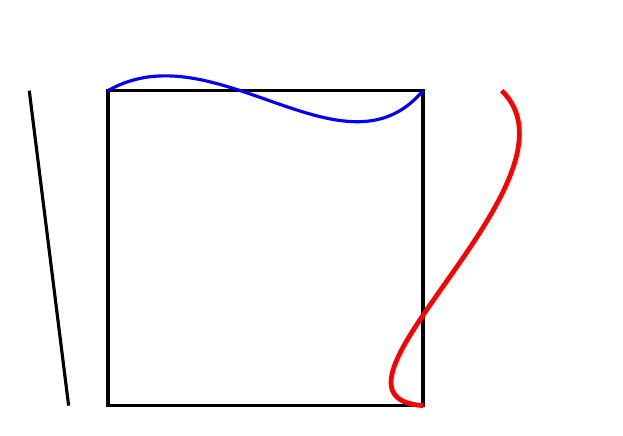
\begin{tikzpicture}
\draw[line width=.4mm](0,0)rectangle(4,4);
\BeamDeformP{0,0}{0,4}{.5}{-1}
\BeamDeformP[blue]{0,4}{4,4}{0}[30]{0}[50]{1}
\setstructmech{linewidth=.6mm}
\BeamDeformP[red]{4,4}{4,0}{.5}[30]{0}[50]{2}
\end{tikzpicture}
\end{figure}
\section{Beam Deformation (Rotation Only)}
\begin{Verbatim}[frame=single,label=Syntax]
\BeamDeformR[1]{2}{3}[4][5]{6}
\end{Verbatim}
\begin{enumerate}
\item[][1] --- optional, line colour.
\item[]\{2\} --- node coordinates of the lower end in form of \Highlight{$x,y$}.
\item[]\{3\} --- node coordinates of the higher end in form of \Highlight{$x,y$}.
\item[][4] --- optional, rotation value of the lower end, can be negative.
\item[][5] --- optional, rotation value of the high end, can be negative.
\item[]\{6\} --- optional, scale.
\end{enumerate}
Caveat: If the nodal translations are expressed as global values, they can be readily combined into parameters \Highlight{\#2} and \Highlight{\#3}, so there is no need to provide another command to plot the deformation in the global coordinate system.
\begin{Verbatim}[frame=single,label=Example]
\BeamDeformR{0,0}{0,4}[50][30]
\BeamDeformR[blue]{0,4}{4,4}[20][30]{2}
\end{Verbatim}
\begin{figure}[H]
\centering
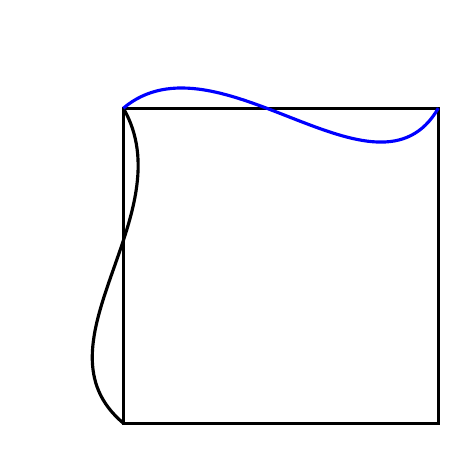
\begin{tikzpicture}
\draw[line width=.4mm](0,0)rectangle(4,4);
\BeamDeformR{0,0}{0,4}[50][30]
\BeamDeformR[blue]{0,4}{4,4}[20][30]{2}
\end{tikzpicture}
\end{figure}
\end{document}